% Data in Brief — Data Article
% Structure follows the Data in Brief article template (January 2026).
% Compile: pdflatex dib_main.tex  (x2). Requires elsarticle.cls (in MacTeX).
% Submission: Editorial Manager, article type "Data Article".
% Before submitting: (1) make the GitHub repo public, (2) mint a Zenodo DOI
% for the release and paste it into the Specifications Table and Data
% Availability, (3) fill the corresponding e-mail, (4) see NOTES at the end.

\documentclass[preprint,12pt]{elsarticle}

\usepackage{amsmath}
\usepackage{booktabs}
\usepackage{array}
\usepackage{graphicx}
\usepackage{url}
\usepackage{hyperref}
\usepackage{longtable}
\usepackage[T1]{fontenc}
\usepackage{lmodern}
\usepackage{microtype}

\journal{Data in Brief}

\begin{document}
\sloppy

\begin{frontmatter}

\title{A campaign-level dataset of 401 GHSA and OSV malware advisories for 200 PyPI and npm packages, with mechanism labels and reporter-coverage annotations}

\author[1]{Tahsin Tajwar Tanni\corref{cor1}}
\ead{CORRESPONDING-EMAIL@example.com} % TODO: fill in
\author[1]{Nafiz Khan}
\cortext[cor1]{Corresponding author.}
\affiliation[1]{organization={Independent Researcher}, city={Dhaka}, country={Bangladesh}}

\begin{abstract}
This dataset is a frozen, checksummed snapshot of 401 confirmed-malicious package advisories for the PyPI and npm ecosystems, collected on 2 October 2026 from the GitHub Security Advisory database (GHSA, 200 records) and OSV.dev (201 records). The 401 records describe 200 distinct packages (100 per ecosystem); 386 of them were published between 1 September and 2 October 2026. Each record carries the advisory identifier, source, package name, ecosystem, summary, full description text, publication timestamp, severity, reference URLs and fetch timestamp. The dataset is accompanied by derived tables produced by a documented, tested pipeline: (i) a two-stage collapse of records into 94 independent attack campaigns (per-package merge of cross-source re-reports, then grouping by reporter-assigned campaign tag or masked description prefix); (ii) a binary \emph{described-mechanism} label per record from a six-category regular-expression taxonomy with a negation guard, together with a 51-row human verification sheet (precision 0.94, 95\% CI 0.83--0.98); (iii) per-package reporter-coverage annotations parsed from the advisories' \texttt{\#\# Source:} headers (reporter count and indicators for kam193, Amazon Inspector and GHSA boilerplate); and (iv) a compound/generic naming flag per package, with its validation against 139 publicly disclosed LLM-hallucinated package names and the top-5,000 packages of each ecosystem. The data support studies of advisory duplication, reporter bias in advisory text, malicious-package naming and the reuse of advisory databases as ground truth. All code, tests and manifests needed to regenerate every derived table from the frozen snapshot are included.
\end{abstract}

\begin{keyword}
software supply chain \sep malicious packages \sep security advisories \sep PyPI \sep npm \sep GHSA \sep OSV \sep measurement validity
\end{keyword}

\end{frontmatter}

% ---------------------------------------------------------------------
\section*{Specifications Table}

\begin{longtable}{>{\raggedright\arraybackslash}p{0.27\textwidth} >{\raggedright\arraybackslash}p{0.68\textwidth}}
\toprule
Subject & Computer Science: Software. \\
\midrule
Specific subject area & Software supply-chain security; malicious open-source packages; security advisory databases; measurement of advisory text as a behavioural label. \\
\midrule
Type of data & Table (JSON Lines, JSON, CSV, Markdown); text (advisory descriptions); processed and analysed derived tables; Python source code and tests. Raw data: advisory records as returned by the GHSA and OSV APIs, deduplicated and frozen. Derived data: campaign assignments, mechanism labels, reporter-coverage annotations, naming-grammar flags, human verification sheet, grammar validation statistics, power-analysis outputs. \\
\midrule
Data collection & Advisories of type \texttt{malware} for the \texttt{pip} and \texttt{npm} ecosystems were retrieved from the GitHub Security Advisory (GHSA) REST API (five pages, newest first, unauthenticated) on 2 October 2026. For every package name found, OSV.dev was queried for its corresponding advisory. Records were deduplicated on (ecosystem, package name, advisory identifier) and written to a single JSON Lines file with a SHA-256 manifest. Labels and annotations were computed from that file only, by scripts included in the repository, using Python 3.14 with pandas, scipy and statsmodels. One author verified 51 labeler positives by reading the advisory text under a written rule. \\
\midrule
Data source location & Primary sources: GitHub Security Advisory database (\url{https://github.com/advisories}, GitHub, Inc., San Francisco, USA) and OSV.dev (\url{https://osv.dev}, Google LLC, Mountain View, USA). Secondary source for grammar validation: the publicly disclosed ``universal'' hallucinated-package-name lists of Churilov~\cite{churilov2026}, release \texttt{v0.2-preprint}, Zenodo DOI 10.5281/zenodo.19859120 (CC~BY~4.0). Benign comparison lists: top-5,000 PyPI downloads (\texttt{hugovk/top-pypi-packages}) and \texttt{npm-high-impact} v1.13.0. Data were collected and processed in Dhaka, Bangladesh. \\
\midrule
Data accessibility & Repository name: Zenodo. \newline
Data identification number: 10.5281/zenodo.XXXXXXX \textbf{[TODO: mint before submission]}. \newline
Direct URL to data: \url{https://doi.org/10.5281/zenodo.XXXXXXX} \newline
Source code (mirror): \url{https://github.com/TahsinTanni/Phantom-Guard} \newline
Instructions for accessing these data: download the Zenodo archive; \texttt{data/frozen/incidents\_snapshot.jsonl} is the raw snapshot; \texttt{python run\_check.py} regenerates the campaign-level tables from it; \texttt{python -m pytest tests/ -q} runs the test suite. \\
\midrule
Related research article & None. \textbf{[TODO: if the companion analysis paper is accepted before this article is submitted, cite it here as the related research article.]} \\
\bottomrule
\end{longtable}

% ---------------------------------------------------------------------
\section*{1. Value of the Data}

\begin{itemize}
\item Advisory databases are increasingly mined as ground truth for what malicious packages do, yet their records are not independent observations: this dataset makes the duplication explicit (401 records $\rightarrow$ 200 packages $\rightarrow$ 94 campaigns) and provides the campaign assignments, so researchers can run tests at the correct unit of analysis.
\item Every advisory text is annotated with the reporters that contributed to it. This allows the effect of reporter coverage on text-derived labels to be measured and controlled, which no public malicious-package dataset currently supports.
\item The snapshot is frozen and checksummed, and every derived table is regenerated from it by tested code, so results computed on it are exactly reproducible even though both source databases change continuously.
\item The 51-row human verification sheet and the written labeling rule give a measured precision for the regex-based mechanism labels, which lets other researchers decide whether to reuse the labels or re-annotate.
\item The naming-grammar validation (hallucinated versus benign versus malicious name sets) is a reusable negative result: a compound-token grammar does not identify LLM-hallucinated package names, which saves others from building on that proxy.
\end{itemize}

% ---------------------------------------------------------------------
\section*{2. Background}

Malicious packages make up a large share of reported vulnerabilities in npm and PyPI~\cite{akhavani2025}, and large language models add a further route to them by recommending packages that do not exist, whose names an attacker can then register~\cite{spracklen2025,huang2026}. Empirical work on this threat commonly treats the GitHub Security Advisory database (GHSA) and OSV as ground truth both for which packages are malicious and for what the malware does. Two assumptions are usually made and rarely tested: that advisory records are independent, and that a mechanism mentioned in the advisory text is a property of the malware rather than of whoever wrote the advisory.

This dataset was assembled to test those assumptions while studying whether compound/generic package naming (e.g.\ \texttt{py-*}, \texttt{*-tools}, \texttt{*-client}) is associated with a described payload mechanism. During that study, the campaign grouping was corrected three times (142 $\rightarrow$ 106 $\rightarrow$ 94 campaigns) as the human verification surfaced merge failures, and the dependence of labels on reporter coverage emerged as the dominant effect. We release the snapshot, the corrected grouping, the labels, the reporter annotations and the verification sheet so that these measurement properties can be reused and the analysis independently repeated or extended.

% ---------------------------------------------------------------------
\section*{3. Data Description}

The repository is organised as a Python project. The files that constitute the dataset are listed below; all paths are relative to the repository root.

\subsection*{3.1 Raw snapshot}

\texttt{data/frozen/incidents\_snapshot.jsonl} --- 401 records, one JSON object per line. Table~\ref{tab:schema} gives the fields. Table~\ref{tab:counts} summarises the composition and Fig.~\ref{fig:timeline} shows the publication dates.

\begin{table}[h]
\centering
\caption{Fields of \texttt{incidents\_snapshot.jsonl}.}
\label{tab:schema}
\small
\begin{tabular}{>{\raggedright\arraybackslash}p{0.22\textwidth} >{\raggedright\arraybackslash}p{0.12\textwidth} >{\raggedright\arraybackslash}p{0.58\textwidth}}
\toprule
Field & Type & Content \\
\midrule
\texttt{advisory\_id} & string & Advisory identifier: \texttt{GHSA-xxxx-xxxx-xxxx} (GHSA), \texttt{MAL-yyyy-nnnn} (OSV malicious-package record), or \texttt{PYSEC-\ldots} (one OSV record). \\
\texttt{source} & string & \texttt{ghsa} or \texttt{osv}. \\
\texttt{package\_name} & string & Package name as registered, including npm scope where present. \\
\texttt{ecosystem} & string & \texttt{pypi} or \texttt{npm}. \\
\texttt{summary} & string & One-line advisory summary. \\
\texttt{description} & string & Full advisory text (Markdown). Median length 1,335 characters (range 216--4,414). OSV texts concatenate per-reporter sections introduced by \texttt{\#\# Source:} headers. \\
\texttt{published\_at} & string & ISO-8601 publication timestamp (UTC). \\
\texttt{withdrawn\_at} & string & Withdrawal timestamp; \texttt{None} for all 401 records. \\
\texttt{severity} & string & \texttt{critical} for GHSA records; empty for OSV records, which carry no severity. \\
\texttt{reference\_urls} & list of strings & Reference URLs attached to the advisory (reporter pages, registry pages). \\
\texttt{fetched\_at} & string & ISO-8601 retrieval timestamp (UTC). \\
\bottomrule
\end{tabular}
\end{table}

\begin{table}[h]
\centering
\caption{Composition of the raw snapshot.}
\label{tab:counts}
\small
\begin{tabular}{lr}
\toprule
Records & 401 \\
\quad from GHSA / from OSV & 200 / 201 \\
\quad PyPI / npm & 201 / 200 \\
Distinct packages (ecosystem, name) & 200 (100 PyPI, 100 npm) \\
Published September 2026 / October 2026 & 304 / 82 \\
Published before September 2026 & 15 (earliest 30 October 2025) \\
Withdrawn & 0 \\
\bottomrule
\end{tabular}
\end{table}

Every package has exactly one GHSA record and one OSV record, except one PyPI package that has two OSV records (a \texttt{MAL-} and a \texttt{PYSEC-} entry); that is why there are 401 rather than 400 records. The accompanying file \texttt{data/metadata/incidents\_snapshot\_manifest.json} records the SHA-256 digest of the snapshot, the record count, the retrieval date, the preprocessing version and the installed package versions.

\begin{figure}[h]
\centering
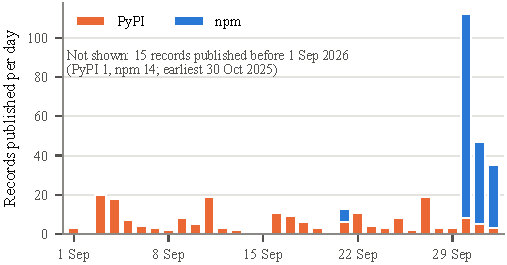
\includegraphics[width=1.0\textwidth]{figures/fig_timeline.pdf}
\caption{Advisory records published per day, 1 September to 2 October 2026, by ecosystem. The npm records cluster in the last three days of the window.}
\label{fig:timeline}
\end{figure}

\subsection*{3.2 Derived campaign-level data}

The two-stage collapse described in Section~4.3 assigns every package to one of 94 campaigns (22 npm, 72 PyPI; Fig.~\ref{fig:units}). The campaign table is regenerated by \texttt{python run\_check.py} and written to \texttt{results/}; it carries, per campaign, the member packages, the ecosystem, the campaign signature, the aggregated naming-grammar flag, the aggregated described-mechanism label, the reporter count and the three reporter indicators. The npm side is dominated by a few families: two WhatsApp-library fork families of 45 and 15 names, a 10-name dependency-confusion family and two related families of 10 and 3 names, which together contain 83 of the 100 npm packages. PyPI campaigns are mostly singletons.

\begin{figure}[h]
\centering
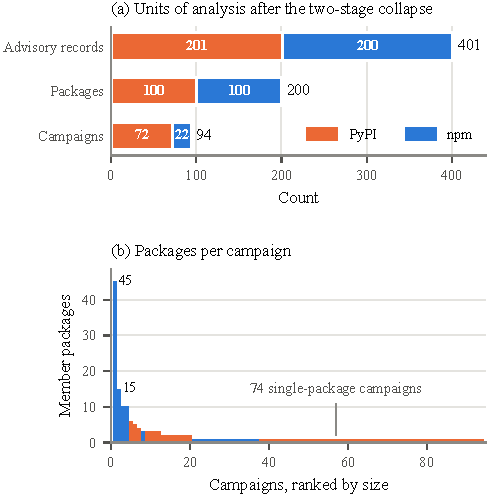
\includegraphics[width=0.85\textwidth]{figures/fig_units.pdf}
\caption{(a) Records, packages and campaigns by ecosystem. (b) Member packages per campaign, ranked by size; 74 of the 94 campaigns contain a single package.}
\label{fig:units}
\end{figure}

\subsection*{3.3 Mechanism labels and human verification}

\texttt{src/labeling/malware\_taxonomy.py} defines six mechanism categories (obfuscated payload execution; hidden install hook; credential or wallet exfiltration; remote backdoor access; remote payload retrieval; brand-impersonation narrative), each as a list of regular expressions with the advisory text that motivated it. The labeler in \texttt{src/labeling/malware\_labeler.py} reads text only, never the package name, which a test enforces. Of the 94 campaigns, 51 are labelled positive under the union of a package's GHSA and OSV texts; Fig.~\ref{fig:mechanisms} gives the count per category.

\texttt{reports/labeler\_spot\_check.md} is the human verification sheet: 51 labeler-positive rows (all 21 packages that are positive only through OSV-carried text, plus 30 sampled campaigns), each with the matched span, the surrounding text, the annotator's verdict (REAL / FALSE / UNSURE) and a note. \texttt{results/spot\_check\_verdicts.json} holds the same verdicts in machine-readable form. The outcome was 44 REAL, 3 FALSE and 4 UNSURE: precision 0.936 (95\% Wilson CI 0.828--0.978) excluding UNSURE, or 0.863 (0.743--0.932) counting UNSURE as FALSE. \texttt{reports/osv\_only\_positives.md} lists the 21 OSV-only positives with their reporter sections.

\begin{figure}[h]
\centering
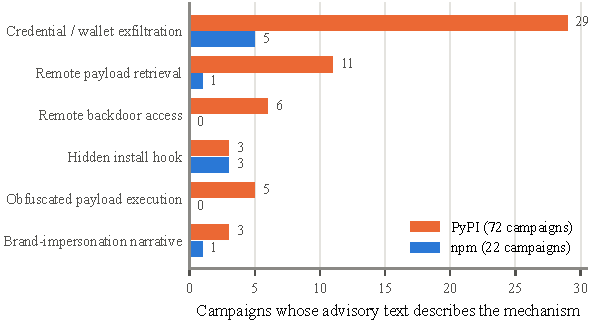
\includegraphics[width=0.9\textwidth]{figures/fig_mechanisms.pdf}
\caption{Campaigns whose advisory text (GHSA and OSV combined) describes each mechanism category, by ecosystem. A campaign can match several categories.}
\label{fig:mechanisms}
\end{figure}

\subsection*{3.4 Reporter-coverage annotations}

For every package, the \texttt{\#\# Source:} headers of both texts are parsed (\texttt{extract\_reporters} in \texttt{src/data/incident\_clients.py}) into a reporter count (\texttt{n\_reporters}) and three indicators: \texttt{kam193}, \texttt{amazon\_inspector} and \texttt{boilerplate} (GHSA's generic ``should be considered fully compromised'' text, which OSV mirrors as a \texttt{ghsa-malware} section; the two count as one reporter). Headerless text without boilerplate is marked \texttt{<unattributed>} (73 of 200 packages). Fig.~\ref{fig:reporters} shows the reporter combinations per package. Among campaigns, the described-mechanism rate (Fig.~\ref{fig:dvrep}) is 0.65 (46/71) with Amazon Inspector coverage against 0.22 (5/23) without, and 0.38 (5/13) for campaigns in which the GHSA boilerplate is one of the reporters; the 4 campaigns whose only reporter is the boilerplate are all mechanism-negative (0/4).

\begin{figure}[h]
\centering
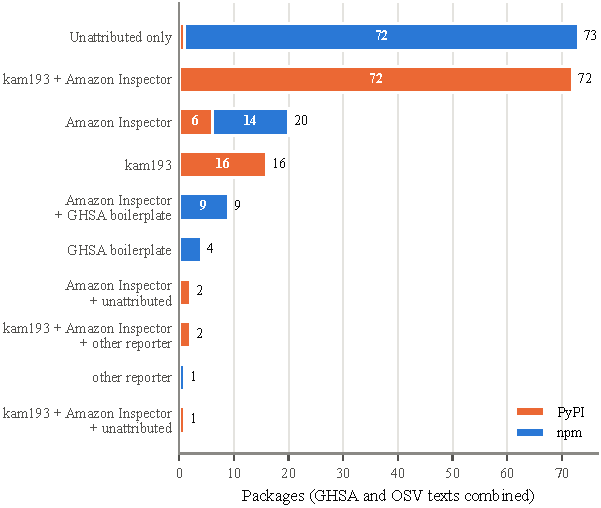
\includegraphics[width=0.95\textwidth]{figures/fig_reporters.pdf}
\caption{Reporter combinations per package, parsed from the \texttt{\#\# Source:} headers of both texts. Most npm packages carry no reporter header; most PyPI packages are covered by both kam193 and Amazon Inspector.}
\label{fig:reporters}
\end{figure}

\begin{figure}[h]
\centering
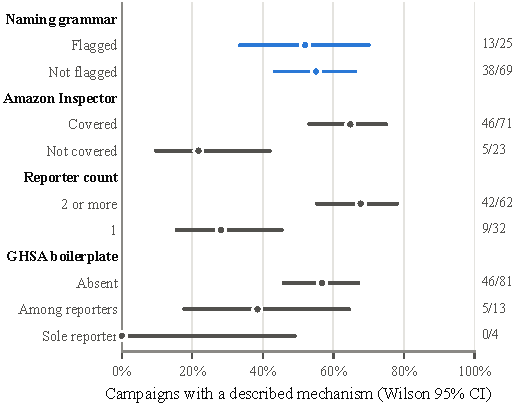
\includegraphics[width=0.8\textwidth]{figures/fig_dv_by_reporter.pdf}
\caption{Share of campaigns labelled mechanism-positive, by naming flag and by reporter coverage (Wilson 95\% CIs; counts at right).}
\label{fig:dvrep}
\end{figure}

\subsection*{3.5 Naming-grammar flag and its validation}

\texttt{src/data/naming\_grammar.py} flags a name that contains a token from lists of compound prefixes, compound suffixes or trend suffixes (e.g.\ \texttt{py-}, \texttt{-tools}, \texttt{-client}, \texttt{-sdk}). \texttt{results/grammar\_validation.json} reports the flag rate on four sets (Table~\ref{tab:grammar}, Fig.~\ref{fig:grammar}). \texttt{data/external/hallucinated\_names.txt} is the 139-name validation set (121 PyPI, 18 npm) with its provenance in \texttt{data/external/hallucinated\_names\_SOURCES.md}.

\begin{table}[h]
\centering
\caption{Naming-grammar flag rate by set, with Wilson 95\% confidence intervals.}
\label{tab:grammar}
\small
\begin{tabular}{lrrl}
\toprule
Set & $n$ & Flagged & Rate [95\% CI] \\
\midrule
LLM-hallucinated names~\cite{churilov2026} & 139 & 7 & 0.050 [0.025, 0.100] \\
Benign top-5,000 PyPI & 5,000 & 821 & 0.164 [0.154, 0.175] \\
Benign top-5,000 npm & 5,000 & 1,031 & 0.206 [0.195, 0.218] \\
Malware campaigns (this dataset) & 94 & 25 & 0.266 [0.187, 0.363] \\
\bottomrule
\end{tabular}
\end{table}

\begin{figure}[h]
\centering
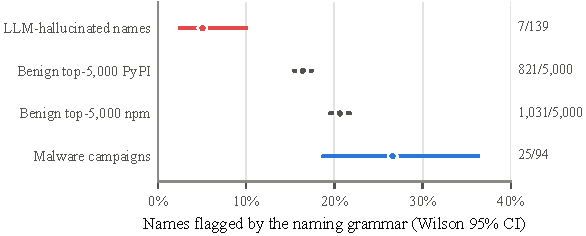
\includegraphics[width=0.8\textwidth]{figures/fig_grammar.pdf}
\caption{Naming-grammar flag rate by set, with Wilson 95\% confidence intervals.}
\label{fig:grammar}
\end{figure}

\subsection*{3.6 Analysis outputs}

\texttt{results/power\_campaign\_level.json} contains the pooled and per-ecosystem $2\times2$ tables, Fisher and Cochran--Mantel--Haenszel results and the power analysis. For reference, the pooled table of grammar flag against described mechanism is $[[13,12],[38,31]]$, odds ratio 0.884 (95\% CI 0.353--2.211), and the design has power 0.31 to detect an odds ratio of 2.0 at $n=94$. \texttt{reports/research\_log.md} is the numbered, dated log of every pipeline change and the numbers it produced, including the superseded groupings.

% ---------------------------------------------------------------------
\section*{4. Experimental Design, Materials and Methods}

\subsection*{4.1 Collection}

The GHSA REST API was queried for advisories with \texttt{type=malware} and ecosystem \texttt{pip} or \texttt{npm}, unauthenticated, newest first, five pages per ecosystem, on 2 October 2026. GHSA is a live API; the five-page window is the reason 386 of 401 records were published in the five weeks before retrieval. For each package name in the GHSA result, OSV.dev was queried by (ecosystem, package) and the returned advisory record stored. Retrieval is checkpointed and resumable (\texttt{src/data/collect\_incidents.py}, \texttt{src/data/incident\_clients.py}).

\subsection*{4.2 Deduplication and freezing}

Records were deduplicated on the key (ecosystem, package name, advisory identifier), preferring GHSA on an exact-key collision and keeping distinct advisory identifiers from either source as separate records. The result was written once to \texttt{incidents\_snapshot.jsonl} and a manifest with its SHA-256 digest was generated (\texttt{src/utils/manifest.py}). All later steps read only this file; the repository's working rules forbid modifying it, and new data must go in a new file with its own manifest.

\subsection*{4.3 Campaign collapse}

Statistical tests on advisories assume independent units. Without collapsing, one npm table in the development history reached an odds ratio of 178 on single-digit cells, driven by one attacker's many package names. The collapse (\texttt{collapse\_to\_campaign\_level} in \texttt{src/statistics/h1\_pilot\_analysis.py}) has two stages. Stage~1 merges all records of the same (ecosystem, package), which removes GHSA/OSV re-reports. Stage~2 groups packages by a campaign signature chosen in priority order: (i) the reporter's own \texttt{Campaign:} identifier when present (assigned by the kam193 reporter); (ii) otherwise the first 200 characters of the description after stripping \texttt{\#\# Source:} headers and masking the package's own name at word boundaries. GHSA's generic boilerplate and kam193's generic install-time pentest template are never used as keys because they are identical across unrelated incidents; packages carrying only such text remain their own unit. A campaign counts as grammar-flagged, or as mechanism-positive, if any member does. The signature rules were revised twice after human reading of sampled rows showed that per-package headers made identical texts look different and that a 10-name family whose texts begin with the package name was never merged; the superseded groupings (142 and 106 campaigns) are preserved in the research log.

\subsection*{4.4 Mechanism labeling}

The six-category taxonomy was derived from advisory text, first from PyPI examples and then extended with npm phrasing (post-install hooks, JavaScript obfuscators, verbs such as \emph{reads} and \emph{POSTs}) after the PyPI-derived patterns matched 0 of about 200 npm records. A negation guard drops a match when a cue (\emph{does not}, \emph{do not}, \emph{did not}, \emph{doesn't}, \emph{no evidence of}) occurs within 40 characters before it, unless \emph{but}, a semicolon or a period intervenes. The label used for the campaign table is computed on the union of a package's GHSA and OSV descriptions; a GHSA-only variant is available through \texttt{run\_check.py --text-source ghsa}. Generic scanner-verdict boilerplate is deliberately not matched, and a regression test enforces this.

\subsection*{4.5 Human verification}

One author read 51 labeler positives under a written rule recorded in the sheet: a match counts as REAL if the surrounding prose describes the mechanism, as FALSE if the match occurs only in an analyst tag list and not in prose, and as UNSURE otherwise. The sample comprised all 21 OSV-only positives, a census of 12 npm campaigns and a seeded random draw of 18 PyPI campaigns. The annotator saw package names; recall was not measured.

\subsection*{4.6 Reporter extraction and grammar validation}

Reporter sections were parsed from the \texttt{\#\# Source:} headers of both texts of each package and merged per campaign. The grammar was validated by running it unchanged over the 139 universal hallucinated names of Churilov~\cite{churilov2026}, the top-5,000 PyPI packages by downloads and the top-5,000 npm packages by dependents; Wilson intervals are reported. An earlier npm control drawn from registry search results for common terms was flagged at 73\% and discarded, because the search terms were themselves grammar tokens.

\subsection*{4.7 Software}

Python 3.14; pandas, scipy, statsmodels, requests. The test suite (\texttt{tests/}, 160 tests) covers the clients, deduplication, manifest generation, grammar, labeler (including the name-blindness and boilerplate rules), collapse and reporter extraction. \texttt{run\_check.py} reproduces the campaign-level tables and the power analysis from the frozen snapshot in one command.

% ---------------------------------------------------------------------
\section*{Limitations}

The snapshot covers a five-week publication window and 200 packages, because GHSA returns advisories newest first and five pages were fetched; it is a temporal convenience sample, not a census. The npm side consists of a few large families plus singletons, so npm-level statistics rest on very few independent units. Mechanism labels come from a regular-expression taxonomy verified by a single annotator on 51 positives, with no inter-annotator agreement and no recall estimate. Reporter coverage is annotated from headers and 37\% of packages remain unattributed. The campaign grouping was corrected three times and further under-merging is possible. The naming-grammar flag measures compound/generic naming, not LLM hallucination. All packages are confirmed malicious; the benign comparison sets are name lists only and are not matched to the malware set.

% ---------------------------------------------------------------------
\section*{Ethics Statement}

The authors have read and follow the ethical requirements for publication in \emph{Data in Brief}. The data consist of publicly published security advisories and package names; no human subjects, animals or personal data are involved. The dataset contains no malicious code, only advisory text describing it. GHSA advisory data are licensed CC~BY~4.0; OSV records carry per-source licences noted in each record's reference URLs; the hallucinated-name list is CC~BY~4.0.

% ---------------------------------------------------------------------
\section*{CRediT authorship contribution statement}

\textbf{Tahsin Tajwar Tanni:} Conceptualization, Methodology, Software, Validation, Formal analysis, Investigation, Data curation, Writing -- original draft, Writing -- review \& editing, Visualization. \textbf{Nafiz Khan:} Conceptualization, Methodology, Software, Investigation, Writing -- review \& editing. % TODO: adjust to reflect actual contributions.

% ---------------------------------------------------------------------
\section*{Acknowledgements}

This work received no external funding.

\section*{Declaration of Competing Interest}

The authors declare that they have no known competing financial interests or personal relationships that could have appeared to influence the work reported in this paper.

% ---------------------------------------------------------------------
\section*{Data Availability}

Phantom Guard: frozen GHSA/OSV malware-advisory snapshot and campaign-level derived data (Original data) (Zenodo), \url{https://doi.org/10.5281/zenodo.XXXXXXX}. % TODO

% ---------------------------------------------------------------------
\section*{Declaration of generative AI and AI-assisted technologies in the manuscript preparation process}

During the preparation of this work the authors used Claude (Anthropic) to assist with code development and with drafting text. After using this tool, the authors reviewed and edited the content as needed and take full responsibility for the content of the publication.

% ---------------------------------------------------------------------
\begin{thebibliography}{9}

\bibitem{churilov2026}
A.~Churilov, The range shrinks, the threat remains: Re-evaluating LLM package hallucinations on the 2026 frontier-model cohort, arXiv:2605.17062 (2026). Data: \url{https://doi.org/10.5281/zenodo.19859120}

\bibitem{akhavani2025}
S.~A. Akhavani, B.~Ousat, A.~Kharraz, Open source, open threats? Investigating security challenges in open-source software, arXiv:2506.12995 (2025). \url{https://doi.org/10.48550/arXiv.2506.12995}

\bibitem{spracklen2025}
J.~Spracklen, R.~Wijewickrama, A.~H.~M.~N. Sakib, A.~Maiti, B.~Viswanath, M.~Jadliwala, We have a package for you! A comprehensive analysis of package hallucinations by code generating LLMs, in: Proc. 34th USENIX Security Symposium, 2025. arXiv:2406.10279.

\bibitem{huang2026}
Z.~Huang, C.~Liu, Z.~Wang, X.~Cui, X.~Deng, M.~Xu, Package hallucinations as phantoms in open-source software supply chains: An empirical security analysis, ACM Trans. Softw. Eng. Methodol. (2026). % TODO: add DOI

\end{thebibliography}

\end{document}

% =====================================================================
% NOTES (delete before submission)
% 1. Do NOT submit this while the MSR Data & Tool Showcase paper on the same
%    dataset is under review; Data in Brief requires the data article to be
%    original and MSR forbids concurrent submission. Use this as the
%    fallback after the MSR decision, or instead of the showcase.
% 2. Zenodo DOI is required at submission (desk check). Make the GitHub
%    repo public, create a GitHub release, enable the Zenodo-GitHub
%    integration, and paste the DOI in the three TODO places.
% 3. Section 3.2 says the campaign table is written to results/. Make sure
%    run_check.py actually exports a per-campaign CSV (e.g.
%    results/campaigns.csv with member packages, signature, flags,
%    n_reporters, indicators). If it does not yet, add that export.
% 4. APC is USD 1,600. Check Elsevier's Research4Life discount for
%    Bangladesh before submitting.
% 5. Data in Brief is single-anonymous: names stay in.
% =====================================================================
